% Options for packages loaded elsewhere
\PassOptionsToPackage{unicode}{hyperref}
\PassOptionsToPackage{hyphens}{url}
%
\documentclass[
]{article}
\usepackage{amsmath,amssymb}
\usepackage{iftex}
\ifPDFTeX
  \usepackage[T1]{fontenc}
  \usepackage[utf8]{inputenc}
  \usepackage{textcomp} % provide euro and other symbols
\else % if luatex or xetex
  \usepackage{unicode-math} % this also loads fontspec
  \defaultfontfeatures{Scale=MatchLowercase}
  \defaultfontfeatures[\rmfamily]{Ligatures=TeX,Scale=1}
\fi
\usepackage{lmodern}
\ifPDFTeX\else
  % xetex/luatex font selection
\fi
% Use upquote if available, for straight quotes in verbatim environments
\IfFileExists{upquote.sty}{\usepackage{upquote}}{}
\IfFileExists{microtype.sty}{% use microtype if available
  \usepackage[]{microtype}
  \UseMicrotypeSet[protrusion]{basicmath} % disable protrusion for tt fonts
}{}
\makeatletter
\@ifundefined{KOMAClassName}{% if non-KOMA class
  \IfFileExists{parskip.sty}{%
    \usepackage{parskip}
  }{% else
    \setlength{\parindent}{0pt}
    \setlength{\parskip}{6pt plus 2pt minus 1pt}}
}{% if KOMA class
  \KOMAoptions{parskip=half}}
\makeatother
\usepackage{xcolor}
\usepackage[margin=1in]{geometry}
\usepackage{graphicx}
\makeatletter
\def\maxwidth{\ifdim\Gin@nat@width>\linewidth\linewidth\else\Gin@nat@width\fi}
\def\maxheight{\ifdim\Gin@nat@height>\textheight\textheight\else\Gin@nat@height\fi}
\makeatother
% Scale images if necessary, so that they will not overflow the page
% margins by default, and it is still possible to overwrite the defaults
% using explicit options in \includegraphics[width, height, ...]{}
\setkeys{Gin}{width=\maxwidth,height=\maxheight,keepaspectratio}
% Set default figure placement to htbp
\makeatletter
\def\fps@figure{htbp}
\makeatother
\setlength{\emergencystretch}{3em} % prevent overfull lines
\providecommand{\tightlist}{%
  \setlength{\itemsep}{0pt}\setlength{\parskip}{0pt}}
\setcounter{secnumdepth}{-\maxdimen} % remove section numbering
\usepackage{booktabs}
\usepackage{wrapfig}
\usepackage{graphicx}
\usepackage{pgf}
\usepackage{float}
\usepackage[calcwidth]{titlesec}
\usepackage{amssymb}
\usepackage{tikz}
\usepackage{amsmath}
\usepackage{color}
\usepackage{subcaption}
\usepackage[font=footnotesize]{caption}
\usepackage[labelfont=bf,textfont=md]{caption}
\usepackage{titling}
\captionsetup[figure]{font=small, skip=0pt}
                                          
\DeclareRobustCommand{\solidline}{\raisebox{2pt}{\tikz{\draw[thick](0,0) -- (0.5,0);}}}
\DeclareRobustCommand{\dashedline}{\raisebox{2pt}{\tikz{\draw[dashed, thick](0,0) -- (0.5,0);}}}                                          

\titleformat*{\section}{\centering\Large\bfseries}
\ifLuaTeX
  \usepackage{selnolig}  % disable illegal ligatures
\fi
\IfFileExists{bookmark.sty}{\usepackage{bookmark}}{\usepackage{hyperref}}
\IfFileExists{xurl.sty}{\usepackage{xurl}}{} % add URL line breaks if available
\urlstyle{same}
\hypersetup{
  hidelinks,
  pdfcreator={LaTeX via pandoc}}

\author{}
\date{\vspace{-2.5em}}

\begin{document}

\section{Orion Star pH Meter Cross Comparison Report}

IISD Experimental Lakes Area Analytical Service Laboratory\\
Sonya Havens\\
2024-06-13

\subsection{Thermo Scientific\textsuperscript{TM} Orion Star\textsuperscript{TM} A211 Benchtop pH Meter}

The Thermo Scientific\textsuperscript{TM} Orion Star\textsuperscript{TM}
A211 Benchtop pH Meter was purchased from Fisher Scientific 23 March
2023 and included the following parts:

\begin{itemize}
\tightlist
\item
  Star A211 pH meter
\item
  8172BNWP ROSS Sure-Flow glass-body pH electrode
\item
  927007MD stainless steel ATC probe
\item
  810199 pH buffer kit
\item
  electrode stand
\item
  100-240V universal power adapter
\item
  computer cable
\end{itemize}

The Thermo Scientific\textsuperscript{TM} Orion Star\textsuperscript{TM}
A211 pH Meter was received 7 April 2023, installed on 12 June 2023, and
used to measure pH in samples collected from 12 June 2023 to 6 September
2023 (\emph{n} = 301) that were also measured on the Fisher Accumet
Benchtop pH Meter. Samples from the Environment and Climate Change
Canada Proficiency Testing study (ECCC-PT) were also analyzed on both
the Orion Star pH meter and the Fisher Accumet pH meter and compared
with ECCC-PT results. Instrument performance data (e.g.~precision
estimates, instrument response stability, and reference sample
comparison) is also provided.

\subsection{Analytical precision}

The analytical precision (\emph{Pr}), which is based on the residuals of
the standard buffers response along the calibration curve, is calculated
for each run using the measured response (mV) of standard buffers and
equations 1 through 3:

Equation 1. \(Pr = (y_d-b)/m\)

where \emph{b} is the y-intercept, \emph{m} is the slope, and
\emph{y\textsubscript{d}} is the signal detection limit, which is
calculated using equation 2.

Equation 2. \(y_d = 3s_y+b\)

where \emph{s\textsubscript{y}} is the residuals between the measured
response (mV) for each standard buffer and the calibration curve
predicted response (mV) for each standard concentration and is
calculated using equation 3.

Equation 3. \(s_y = √((∑d_i^2 )/(n-2))\)

where \emph{n} is the number of standards in the calibration curve, and
\emph{d\textsubscript{i}} is the difference between the measured
response (mV) for each standard buffer and the calibration curve
predicted response (mV) for each standard buffer.

The average analytical precision of pH measured on the Orion Star pH
meter and Fisher Accumet pH meter during the cross comparison period (14
March 2023 to 3 November 2023) were similar (0.05 ± 0.03 SU, \emph{n} =
36 and 0.03 ± 0.03 SU, \emph{n} = 87, respectively).

\subsection{Replication precision}

Sample replicates are conducted every 15 to 20 samples. The average
relative percent difference (RPD) of replicated samples, calculated
using equation 4, was 0.2\% ± 0.1\% (max = 0.3\%, \emph{n} = 16) and
0.3\% ± 0.4\% (max = 2.6\%, \emph{n} = 81) for replicated samples on the
Orion Star pH meter and on the Fisher Accumet pH meter, respectively.

Equation 4. \(RPD = ((C_1-C_2)/((C_1+C_2)/2)) x 100\)

where \emph{C\textsubscript{1}} and \emph{C\textsubscript{2}} are the
concentrations of the two replicates.

\subsection{Millivolt stability and calibration slope}
\begin{figure}[h]
  \vspace{-0.4cm}
  \begin{subfigure}{0.48\textwidth}
  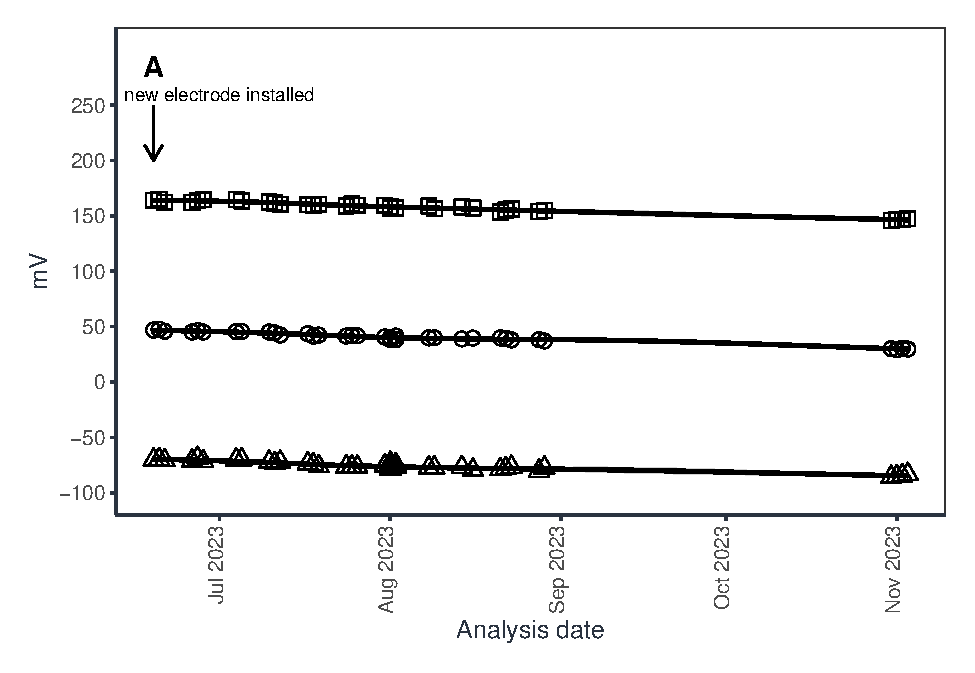
\includegraphics[]{orion_mV.pdf}
  \end{subfigure}%
  \begin{subfigure}{0.48\textwidth}
  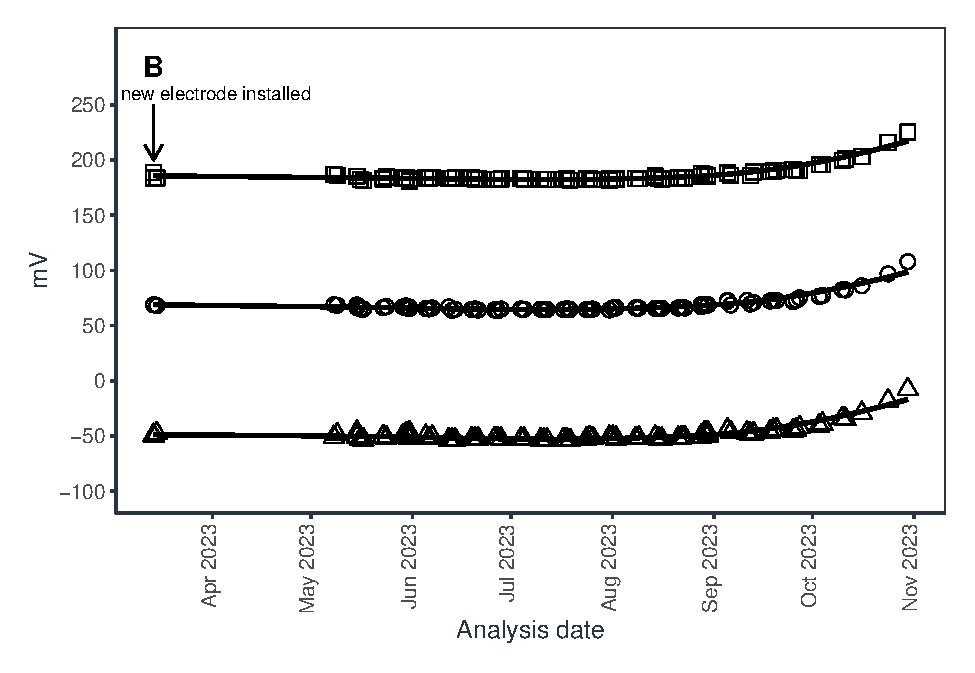
\includegraphics[]{fisher_mV.pdf}
  \end{subfigure}
\caption{pH meter signal response (mV) of pH 4 ($\square$), pH 6 ($\bigcirc$), and pH 8 ($\bigtriangleup$) buffers on the Orion Star pH meter from 19 June 2023 to 3 November 2023 (A) and on the Fisher Accumet pH meter from 14 March 2023 to 30 October 2023 (B).}
\end{figure}

\begin{wrapfigure}[18]{r}{0.45\textwidth}
  \vspace{-0.6cm}
  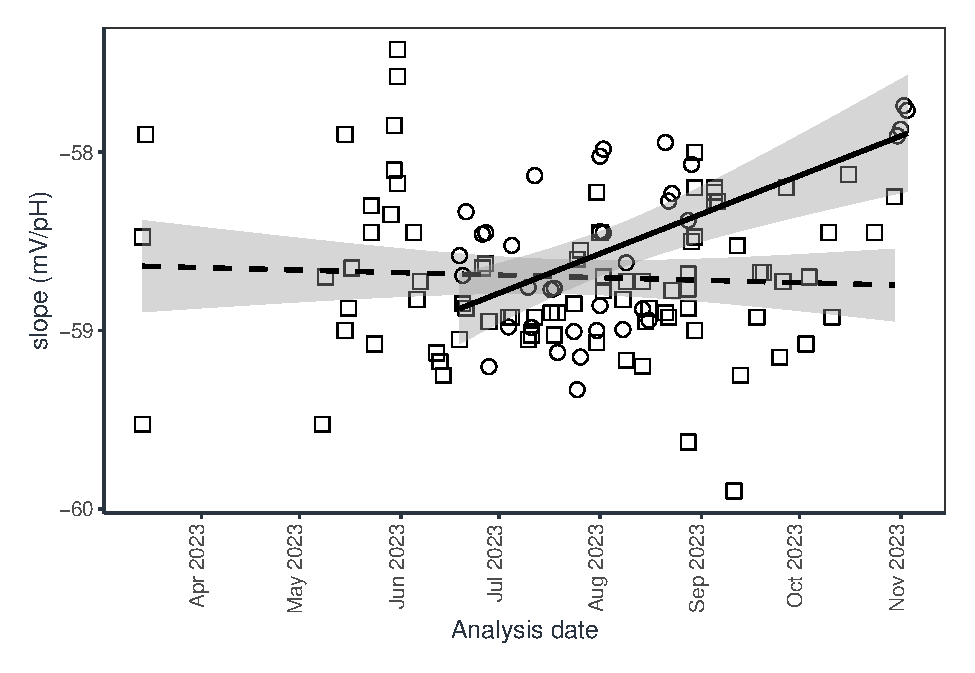
\includegraphics[width=0.45\textwidth]{mV_slope.pdf}
  \caption{Slope of pH meter calibrations of analytical runs on the Orion Star pH meter ($\bigcirc$, \protect\solidline, $\mbox{\textit{y}=0.0049}$$\textit{x}$$\mbox{-155}$, $\mbox{\textit{n}=40}$) from 19 June 2023 to 3 November 2023 and with the Fisher Accumet pH meter ($\square$, \protect\dashedline, $\mbox{\textit{y}=0.0003}$$\textit{x}$$\mbox{-65}$, $\mbox{\textit{n}=40}$) from 14 March 2023 to 30 October 2023.}
\end{wrapfigure}

The millivolt (mV) pH meter response values were stable throughout the
cross comparison study on the Orion Star pH meter, while the mV values
were stable until mid-September on the Fisher Accumet pH meter, at which
point the mV values of each pH buffer started to increase. The
literature established mV values for pH 4, 6, and 8 are 177, 59, and
-59, respectively. The average mV values for pH 4, 6, and 8 were 158 ±
5, 41 ± 5, and -76 ± 4 (\emph{n} = 36), respectively, on the Orion Star
pH meter, which were lower than literature established values by 19 ± 5,
18 ± 5, and 17 ± 4, on average. The average mV values for pH 4, 6, and 8
on the Fisher Accumet pH meter (186 ± 7, 69 ± 7, and -48 ± 7,
respectively, \emph{n} = 87), were higher than established values by 9 ±
7, 10 ± 7, and 11 ± 7, on average, but closer to literature established
values than those measured on the Orion Star pH meter.

Despite the stability of the mV values of pH buffers measured on the
Orion Star pH meter, the slope of the calibration curve increased over
time (Figure 2). The slope started out near the ``ideal'' slope of -59
mV/pH, then slowly increased to \textasciitilde-58 mV/pH. The slope of
the calibration curve on the Fisher Accumet pH meter was stable over
time (Figure 2), however, there was more variability in the slopes of
the Fisher Accumet calibrations (\emph{R\textsuperscript{2}} = 0.0008)
than in the slopes of the Orion Star calibrations
(\emph{R\textsuperscript{2}} = 0.0795). \pagebreak

\subsection{Reference samples}

\begin{wrapfigure}[17]{r}{0.45\textwidth}
  \vspace{-0.7cm}
  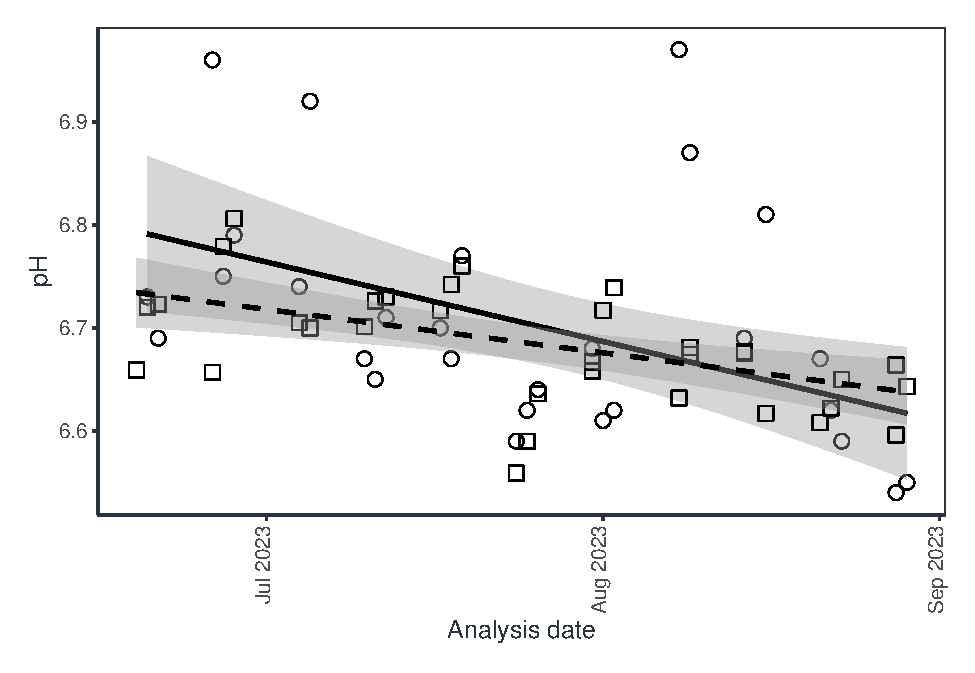
\includegraphics[width=0.45\textwidth]{ref_comparison_date.pdf}
  \caption{The pH of reference sample measured with the Orion Star pH meter ($\bigcirc$, \protect\solidline, $\mbox{\textit{y}=-0.0025}$$\textit{x}$$+$$\mbox{55}$, $\mbox{\textit{n}=35}$) and with the Fisher Accumet pH meter ($\square$, \protect\dashedline, $\mbox{\textit{y}=-0.0014}$$\textit{x}$$+$$\mbox{33}$, $\mbox{\textit{n}=36}$) from June 2023 to September 2023.}
\end{wrapfigure}

A reference sample is included in each analytical run. The average pH
result of reference samples measured on the Orion Star and Fisher
Accumet were similar (6.69 ± 0.12, \emph{n} = 40 and 6.68 ± 0.06,
\emph{n} = 40, respectively). The pH of the reference sample, measured
by both the Orion Star and Fisher Accumet pH meters, slowly declined
over time (Figure 3). This was likely due to CO\textsubscript{2}
dissolution into the reference sample bottle. The reference sample is
lake 239 epilimnetic water that has been aged for at least one year
prior to use so that the chemical constituents can stabilize and come to
equilibrium with the atmosphere. These reference sample pH results
reveal that the sample must not be equilibrated with the atmosphere,
which is likely due to the large volume of the sample. Going forward the
sample should be stored with a large head space and shaken before use to
ensure that the sample is equilibrated with the atmosphere.

The pH results of reference samples were not well correlated among the
two pH meters (Figure 4, \emph{R\textsuperscript{2}} = 0.05,
\emph{p}\textgreater{} 0.01) with the pH measured on the Orion Star pH
meter ranging from 6.54 to 6.97 and the pH measured on the Fisher
Accumet pH meter ranging from 6.56 to 6.81.

Five pH measurements of the reference sample using the Orion Star pH
meter were higher (pH \textgreater{} 6.8) than what would be expected by
the long-term trend (Figure 3). These outliers did not correspond to
elevated analytical precision values or out of range calibration slopes.
When these five outliers are removed, the correlation between pH
measured on the Orion Star pH meter and the Fisher Accumet pH meter is
improved (\emph{R\textsuperscript{2}} = 0.48) and is statistically
significant (\emph{p} \textless{} 0.01). However, the slope of the
linear model (0.76) indicates there is a bias, wherein the Fisher
Accumet pH meter had higher pH value than those witnessed on the Orion
Star pH meter.

Despite the bias, the maximum RPD between the pH measured using the
Orion Star and the Fisher Accumet pH meters was 5\%, with an average RPD
of 1.2\% ± 1.3\%.

\restylefloat*{figure}
\begin{figure}[hb]
  \begin{minipage}[t]{0.48\textwidth}
    \centering
    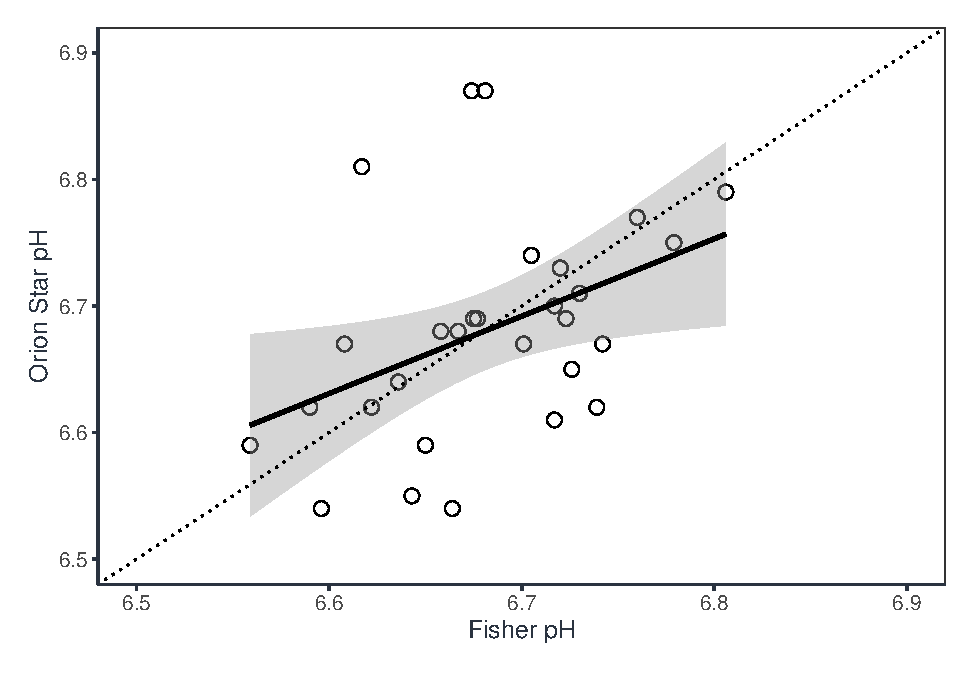
\includegraphics[width=0.98\textwidth]{ref_comparison.pdf}
    \caption{Comparison of pH results of reference sample measured with the Orion Star pH meter and with the Fisher Accumet pH meter ($\mbox{\textit{y}=0.44}$$\textit{x}$$+$$\mbox{4}$, $\mbox{\textit{n}=32}$, $\textit{R}$$^2$$\mbox{=0.05}$, $\mbox{\textit{p} > 0.01}$) from June 2023 to September 2023.}
  \end{minipage}
  \hfill
  \begin{minipage}[t]{0.48\textwidth}
    \centering
    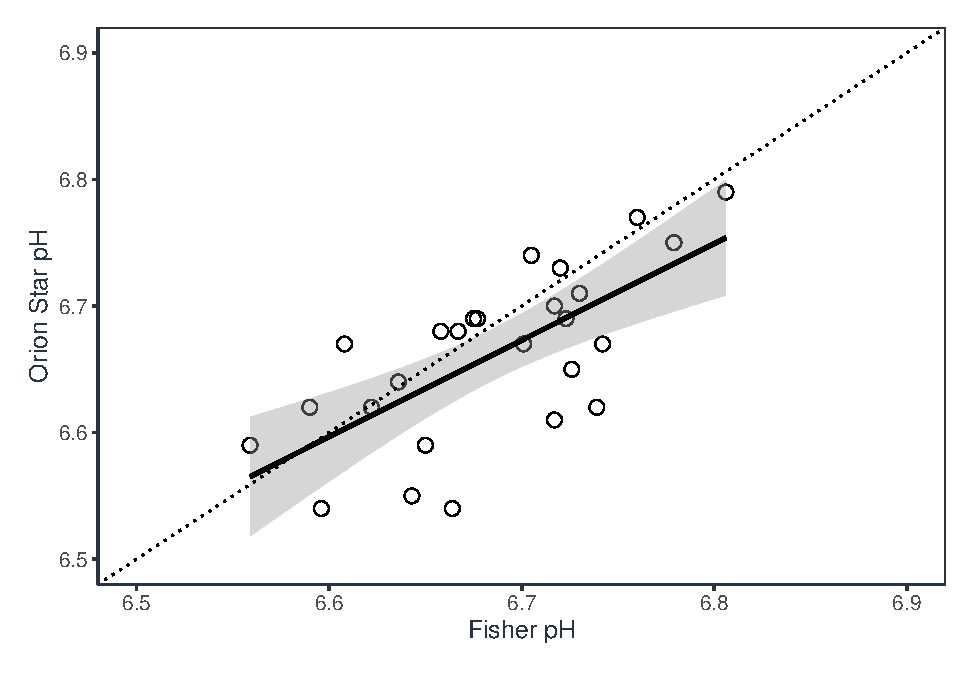
\includegraphics[width=0.98\textwidth]{ref_comparison_no_outliers.pdf}
    \caption{Comparison of pH results of reference sample measured with the Orion Star pH meter and with the Fisher Accumet pH meter from June 2023 to September 2023, with outliers (pH > 6.8) removed ($\mbox{\textit{y}=0.76}$$\textit{x}$$+$$\mbox{2}$, $\mbox{\textit{n}=26}$, $\textit{R}$$^2$$\mbox{=0.48}$, $\mbox{\textit{p} < 0.01}$).}
  \end{minipage}
\end{figure}
\pagebreak

\subsection{Proficienty testing samples}

The pH results from the Environment and Climate Change Canada
Proficiency Testing (ECCC-PT) program were significantly correlated with
those obtained from the Orion Star pH meter and the Fisher Accumet pH
meter (Figure 6). While the 95\% confidence intervals for the slopes of
the ECCC-PT versus Orion Star pH meter and the Fisher Accumet linear
models were the same (between 0.97 and 1.06), the linear regression
lines fall below the 1:1 line, indicating a bias wherein ECCC-PT pH
results were consistently higher than pH results obtained from the Orion
Star pH meter and the Fisher Accumet pH meter (Figure 6). The average
RPD between the ECCC-PT pH and the Orion Star pH was 2.5\% ± 1.4\% (max
= 4.9\%, \emph{n} = 20) and was 2.5\% ± 1.3\% (max = 4.9\%, \emph{n} =
20) between the ECCC-PT pH and the Fisher Accumet pH. The pH results of
ECCC-PT samples measured with the Orion Star pH meter and with the
Fisher Accumet pH meter were significantly correlated (Figure 7) with a
1:1 ratio (95\% confidence interval for the slope of the Fisher Accumet
versus Orion Star linear model was between 0.96 and 1.03).

\restylefloat*{figure}
\begin{figure}[h]
  \begin{minipage}[t]{0.48\textwidth}
    \centering
    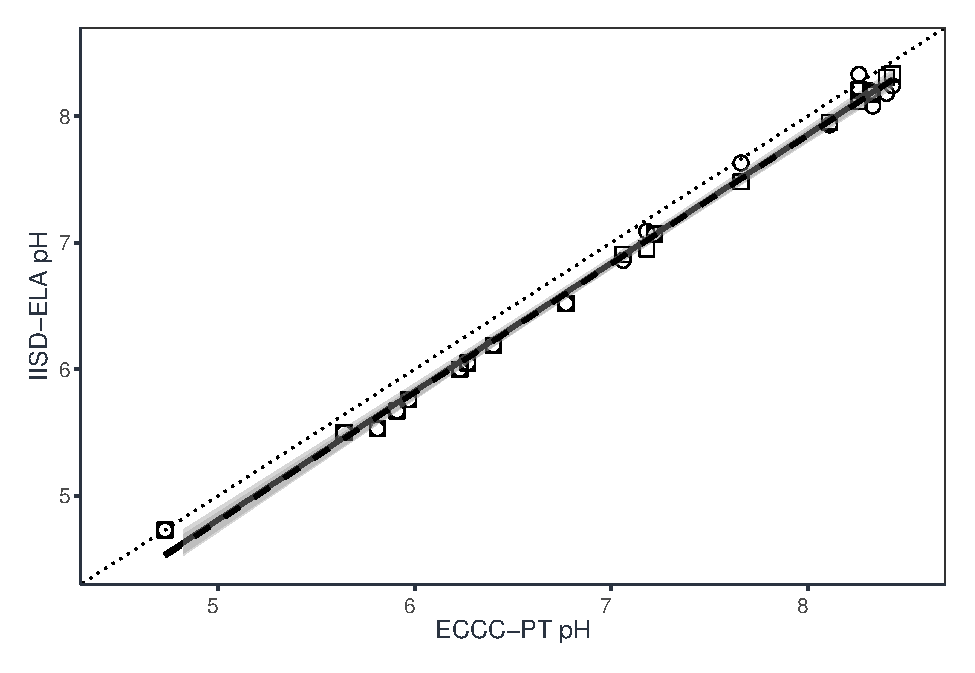
\includegraphics[width=0.98\textwidth]{pt_plot.pdf}
    \caption{Comparison of pH results from the Environment and Climate Change Canada Proficiency Testing (ECCC-PT) program and those obtained from the Orion Star pH meter ($\bigcirc$, \protect\solidline, $\mbox{\textit{y}=1.01}$$\textit{x}$$+$$\mbox{0}$, $\mbox{\textit{n}=20}$, $\textit{R}$$^2$$\mbox{=0.99}$, $\mbox{\textit{p} < 0.001}$) and from the Fisher Accumet pH meter ($\square$, \protect\dashedline, $\mbox{\textit{y}=1.01}$$\textit{x}$$+$$\mbox{0}$, $\mbox{\textit{n}=20}$, $\textit{R}$$^2$$\mbox{=0.99}$, $\mbox{\textit{p} < 0.001}$.}
  \end{minipage}
  \hfill
  \begin{minipage}[t]{0.48\textwidth}
    \centering
    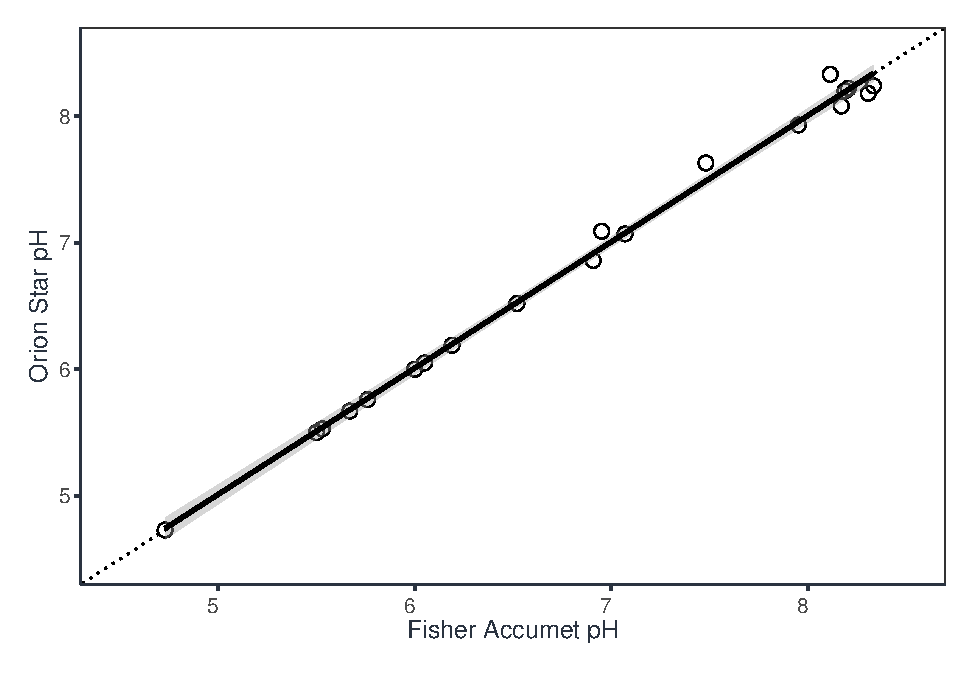
\includegraphics[width=0.98\textwidth]{fisher_v_orion_pt.pdf}
    \caption{Comparison of pH results of Environment and Climate Change Canada Proficiency Testing samples measured with the Orion Star pH meter and with the Fisher Accumet pH meter ($\mbox{\textit{y}=1}$$\textit{x}$$+$$\mbox{0}$, $\mbox{\textit{n}=20}$, $\textit{R}$$^2$$\mbox{=1}$, $\mbox{\textit{p} < 0.001}$).}
  \end{minipage}
\end{figure}

\subsection{Comparison with Fisher Accumet pH results}

\begin{wrapfigure}[16]{r}{0.45\textwidth}
  \vspace{-0.63cm}
  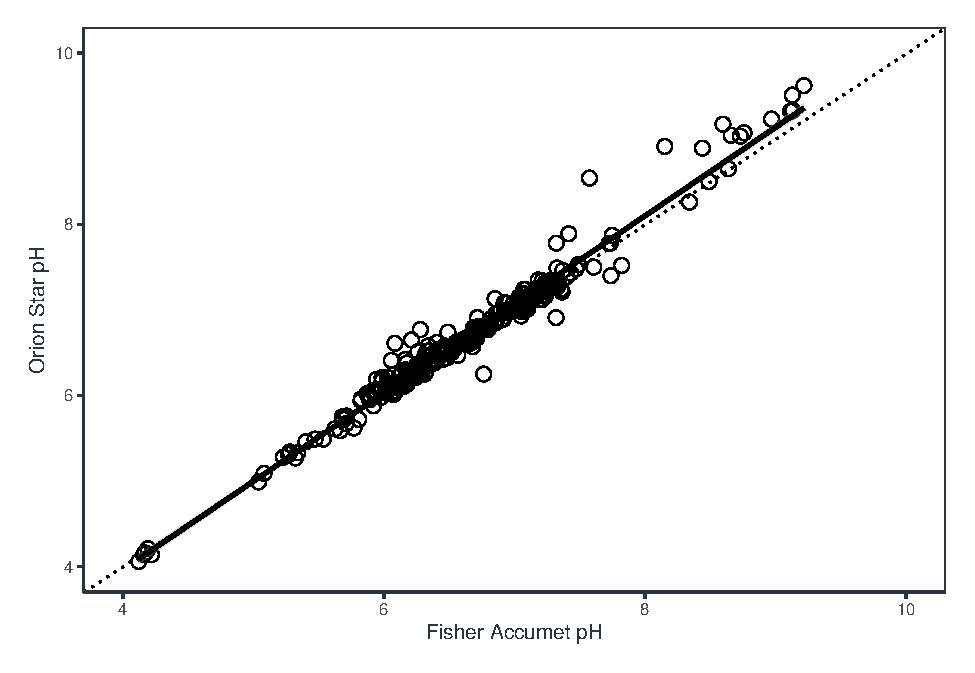
\includegraphics[width=0.45\textwidth]{fisher_v_orion.pdf}
  \caption{Comparison of pH results of samples measured on the Fisher Accumet pH meter and the Orion Star pH meter, $\mbox{\textit{y}=1.03}$$\textit{x}$$\mbox{-0.18}$, $\mbox{\textit{n}=301}$, $\textit{R}$$^2$$\mbox{=0.97}$, $\mbox{\textit{p} < 0.001}$.}
\end{wrapfigure}

The pH of samples measured on the Orion Star pH meter and on the Fisher
Accumet pH meter were significantly correlated (Figure 8,
\emph{R\textsuperscript{2}} = 0.97, \emph{p} \textless{} 0.001). The
95\% confidence interval for the slope of the Fisher Accumet pH meter
versus Orion Star pH meter linear model for pH was between 1.01 and
1.05, indicating that there is a slight bias, wherein the pH measured
using the Orion Star pH meter was slightly higher than when measured
using the Fisher Accumet pH meter (Figure 8). This bias occurred
primarily at pH above 8 (Figure 9). There is no bias when only samples
with pH below 8 are considered (Figure 10) and the 95\% confidence
interval for the slope of the Fisher Accumet pH meter versus Orion Star
pH meter linear model for pH below 8 was between 0.96 and 1.

Regardless of this bias, the average RPD between pH measured using the
Orion Star pH meter and measured using the Fisher Accumet pH meter was
only 1.3\% ± 1.6\%. There were 12 out of 301 samples (4\%) with an RPD
above 5.0\%. The high RPD in the two samples with the highest RPD (12\%
and 8.9\%) was likely due to differences in the pH meter calibrations.
The Fisher Accumet pH meter was calibrated with pH 4, 7, and 10, whereas
the Orion Star pH meter was calibrated with pH 4, 6, 7, and 8 and these
two samples had a pH above 8. The average RPD of samples with pH above 8
was 4\% ± 3.2\%, with a maximum RPD of 12\%, whereas the average RPD of
samples with pH below 8 was 1.1\% ± 1.3\%, with a maximum RPD of 8.3\%.

\restylefloat*{figure}
\begin{figure}[h]
  \begin{minipage}[t]{0.48\textwidth}
    \centering
    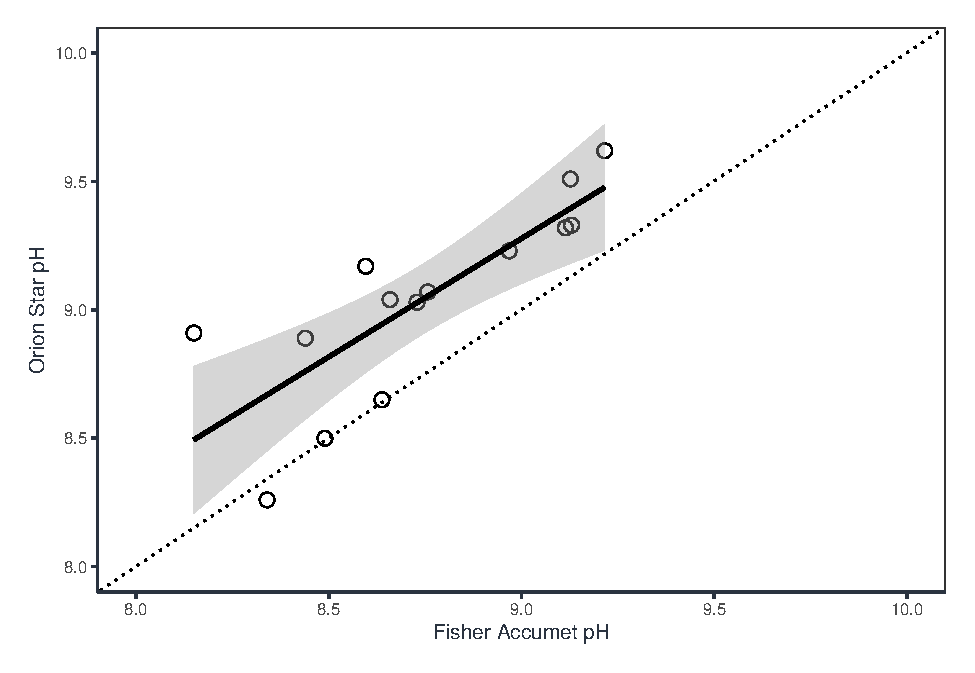
\includegraphics[width=0.98\textwidth]{fisher_v_orion_above_8.pdf}
    \caption{Comparison of pH results of samples measured on the Fisher Accumet pH meter and the Orion Star pH meter in samples with pH above 8, $\mbox{\textit{y}=0.69}$$\textit{x}$$+$$\mbox{3.04}$, $\mbox{\textit{n}=15}$, $\textit{R}$$^2$$\mbox{=0.61}$, $\mbox{\textit{p} < 0.001}$.}
  \end{minipage}
  \hfill
  \begin{minipage}[t]{0.48\textwidth}
    \centering
    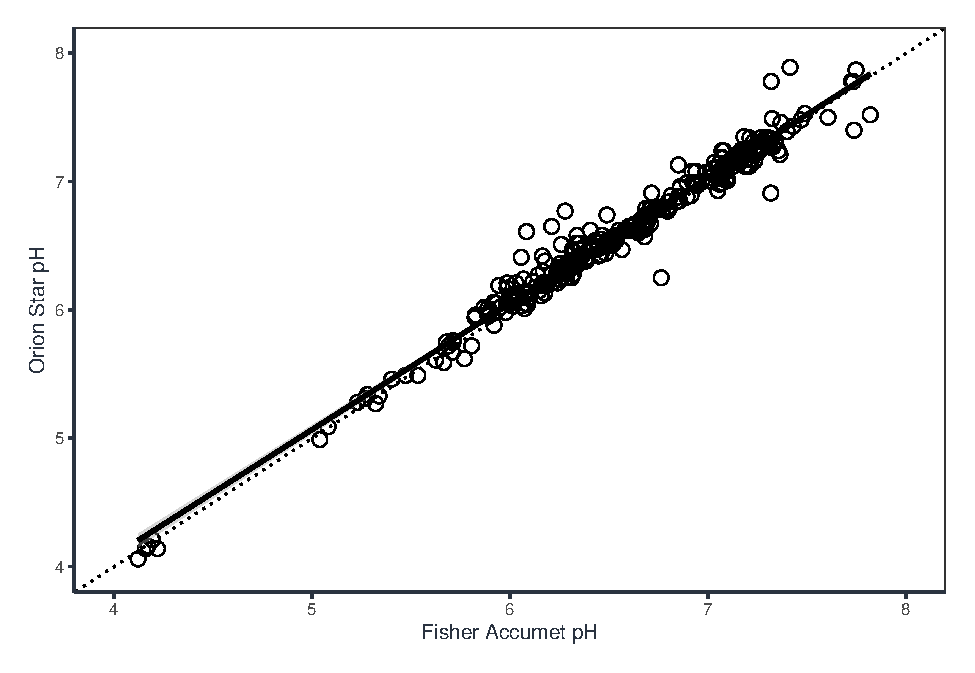
\includegraphics[width=0.98\textwidth]{fisher_v_orion_below_8.pdf}
    \caption{Comparison of pH results of samples measured on the Fisher Accumet pH meter and the Orion Star pH meter in samples with pH below 8, $\mbox{\textit{y}=0.98}$$\textit{x}$$+$$\mbox{0.16}$, $\mbox{\textit{n}=286}$, $\textit{R}$$^2$$\mbox{=0.97}$, $\mbox{\textit{p} < 0.001}$.}
  \end{minipage}
\end{figure}

\subsection{Conclusions}

The Orion Star pH meter had similar analytical and replication precision
as the Fisher Accumet pH meter. The Orion Star electrode is stable over
the course of a field season, as witnessed by the stability of the mV
response. The reference sample pH, measured by both pH meters, decreased
over the course of the field season, which was likely due to
CO\textsubscript{2} dissolution into the sample. To mitigate this,
protocols to ensure that the reference sample is equilibrated with the
atmosphere prior to use will be enacted, which include storing the
sample with a large head space and shaking the sample. While there was a
bias in the reference sample pH, wherein the Fisher Accumet pH meter
generated higher pH on average, this assessment was over a small pH
range (i.e.~6.54 to 6.97) and the RPDs were \(\leq\) 5\%. The Orion Star
pH meter performed within acceptable limits for the measurement of
proficiency testing samples (RPD \(\leq\) 4.9). There was a bias in
samples with a pH above 8, wherein the Orion Star pH meter resulted in
higher pH than the Fisher Accumet pH meter, some of which was due to
differences in the pH meter calibration curve ranges. In previous years,
the Fisher Accumet pH meter was always calibrated with pH buffers 4, 6,
and 8. Going forward, the Orion Star pH meter will calibrated with pH
buffers 4, 6, 8, and 10 rather than 4, 6, 7, and 8, to improve the
accuracy and precision of samples with pH above 8. Despite this bias in
samples with pH above 8, the pH of samples measured on the Orion Star pH
meter were significantly correlated (\emph{R\textsuperscript{2}} = 0.97,
\emph{p} \textless{} 0.001) and 96\% of samples had a RPD \(\leq\)
5.0\%.

\end{document}
